% !TeX root = ../main.tex
\chapter{State of the Art}
\label{CH_2_State of the Art}

\section{Manual And teach pendant based robot programming.}
\label{Manual And teach pendant based robot programming}

Industrial robot programming has traditionally relied on teach pendant-based approaches, where robot motions are explicitly defined and programmed directly during operation. In this method, the programmer manually guides the robot to a sequence of target positions and records these positions using manufacturer-specific programming languages. This approach remains widely used due to its reliability and direct interaction with real-world systems \cite{Siciliano2016Robotics}.

However, teach pendant programming requires substantial expertise in robot kinematics, tooling, and process constraints. Even minor changes in part geometry, fixture placement, or cell layout often require extensive manual reprogramming, leading to increased commissioning effort and system downtime. Consequently, this approach scales poorly in flexible manufacturing environments characterised by frequent product changes and small batch sizes.

In robotic sheet metal handling and press brake applications, these limitations become more pronounced. Large and flexible workpieces introduce additional challenges related to reachability, collision avoidance, and process sequencing. Each step of the bending operation requires the programmer to manually define intermediate robot positions, making the process highly dependent on operator expertise. This often results in iterative trial-and-error adjustments during commissioning \cite{Aomura2002RoboticBending}.

Furthermore, conventional teach pendant programming lacks the level of abstraction required for modern industrial applications that demand rapid reconfiguration and adaptability \cite{Siciliano2016Robotics}. Programs created using this approach are typically tightly coupled to specific robot models, cell configurations, and individual programming styles, which reduces portability and maintainability.

As a result, manual teach pendant programming is generally unsuitable for advanced automation tasks that require high flexibility, integration of process knowledge, and reduced human intervention. These limitations highlight the need for higher-level and more automated programming approaches, which are discussed in the following sections.
%%%%%%%%%%%%%%%%%%%%%%%%%%%%%%%%%%%%%%%%%%%%%%%%%%%%%%%%%%%%%%%%%%
\section{Offline programming approaches for industrial robots}  
\label{Offline programming approaches for industrial robots}


The limitations associated with manual teach pendant programming have led to the widespread adoption of offline programming approaches in industrial robotics. Offline programming enables the development and validation of robot programs within a virtual environment, using digital models of robots, tools, grippers, and workpieces, without interrupting ongoing production \cite{Siciliano2016Robotics}.

This approach is typically based on computer-aided design (CAD) and computer-aided manufacturing (CAM) models, which provide geometric representations of the robot, the workpiece, and the surrounding environment. These models allow robot trajectories and task sequences to be simulated and verified prior to deployment in the physical system. As a result, offline programming reduces commissioning time and improves safety by enabling early detection of potential issues such as reachability limitations and collisions \cite{Pan2012Survey}.

In robot-assisted sheet metal handling and press brake operations, offline programming is commonly used to generate robot programs for tasks such as sheet handling, bending sequences, and intermediate regripping operations. Through virtual simulation, engineers can evaluate the feasibility of robot motions, validate bending sequences, and identify potential conflicts with tooling or fixtures \cite{Aomura2002RoboticBending}.

Despite these advantages, offline programming has several limitations. Its effectiveness depends heavily on the accuracy of the digital model. Any discrepancy between the virtual model and the physical system, such as calibration errors, fixture misalignment, or changes in tool geometry, can lead to incorrect robot behaviour during execution. In such cases, additional manual adjustments and reprogramming are required during commissioning.

Furthermore, offline programming is less suitable for production environments with frequent changeovers and high product variability. Robot programs are typically developed for specific part geometries and process conditions, which limits their adaptability. In multi-stage bending operations, regripping and repositioning steps must still be manually defined and validated by engineers, increasing development effort and reducing flexibility \cite{Pan2012Survey,Aomura2002RoboticBending}.

In summary, offline programming provides significant improvements over manual programming by enabling virtual validation and reducing on-site teaching effort. However, its reliance on accurate digital models and manually defined task sequences limits its effectiveness in highly flexible manufacturing scenarios. These limitations indicate the need for higher-level and more automated robot programming approaches, which are discussed in the following section.
%%%%%%%%%%%%%%%%%%%%%%%%%%%%%%%%%%%%%%%%%%%%%%%%%%%%%%%%%%%%%%%%%%%
\section{Automatic and Rule-Based Robot Program Generation}
\label{Automatic and Rule-Based Robot Program Generation}


To further reduce the engineering effort associated with manual and offline programming, research in industrial robotics has increasingly focused on automatic robot program generation. These approaches aim to derive executable robot programs from high-level task descriptions and geometric information, thereby minimising the need for direct human intervention \cite{Siciliano2016Robotics,Pan2012Survey}.

A prominent approach within this domain is rule-based and task-level programming. In such methods, predefined rules or structured task descriptions are used to resolve constraints related to robot kinematics, tool orientation, and process feasibility. This enables the robot to execute recurring industrial tasks in a consistent and systematic manner while reducing operator involvement \cite{Pan2012Survey,Kruger2009SkillBasedRobotics}.

Many systems adopt reusable motion primitives or skill-based representations as the foundation for automatic program generation. Instead of programming individual joint motions, higher-level actions such as grasping, approaching, or repositioning are defined as modular components. These components can be combined to form complex task sequences, improving modularity, scalability, and reusability in robot programming \cite{Kruger2009SkillBasedRobotics,Schou2013SkillBasedProgramming}.

Automatic program generation is often supported by geometric and feature-based representations of workpieces, typically derived from CAD models. These representations allow the system to automatically identify relevant features, such as edges, surfaces, or grasping regions, and to generate corresponding task sequences and approach strategies. Compared to manual and offline programming, this approach improves adaptability to different product variants and reduces programming effort \cite{Bjorkelund2012KnowledgeBasedProgramming}.

These methods have also been applied to robotic sheet metal handling and press brake automation. In such systems, bending sequences, grasp configurations, and placement strategies can be derived from geometric constraints and process requirements rather than manual teaching. This reduces engineering effort and improves consistency for repetitive tasks involving similar workpieces \cite{Aomura2002RoboticBending,Gupta1998SheetMetalBending}.

Despite these advantages, rule-based program generation approaches exhibit several limitations. Most systems rely on predefined rules and assumptions regarding part geometry, fixture layout, and process conditions, which restrict their applicability in highly variable production scenarios. As task complexity increases, the number of rules also grows, making the system more difficult to maintain, scale, and validate \cite{Siciliano2016Robotics,Kruger2009SkillBasedRobotics}.

In the context of sheet metal bending, regripping operations remain a significant challenge. Multi-stage bending often requires the workpiece to be repositioned using an orientation table, followed by regrasping in a new configuration. Existing approaches typically rely on predefined regripping strategies tailored to specific tools and cell layouts, limiting their general applicability \cite{Aomura2002RoboticBending,Gupta1998SheetMetalBending}.

Furthermore, although automatic grasp planning and trajectory generation methods have been investigated, they are often developed independently and are not fully integrated into a unified planning framework for industrial press brake systems. This lack of integration limits the ability to handle complex, multi-stage manipulation tasks involving both grasp planning and reorientation.

In addition to task-level planning, trajectory generation plays a critical role in translating high-level robot actions into executable motion. Industrial robot systems typically rely on interpolation-based trajectory generation, where motion between poses is discretised into intermediate waypoints to ensure smooth and continuous execution \cite{Biagiotti2008Trajectory, Siciliano2016Robotics}. These approaches ensure that the robot follows controlled Cartesian paths and avoids abrupt changes in motion. However, many industrial implementations treat trajectory generation as a low-level controller function, with limited integration into higher-level planning strategies. This separation can reduce flexibility when adapting to complex handling tasks such as regripping and multi-stage manipulation.

In summary, automatic and rule-based programming approaches significantly reduce engineering effort and improve consistency compared to traditional methods. However, their reliance on predefined rules and limited adaptability highlights the need for more integrated and flexible solutions, particularly for applications such as robotic sheet metal bending. These challenges are further examined in the following section.
%%%%%%%%%%%%%%%%%%%%%%%%%%%%%%%%%%%%%%%%%%%%%%%%%%%%%%%%%%%%%%%%%%%%
\section{Robotic Sheet-Metal Bending and Press-Brake Cells}
\label{Robotic Sheet-Metal Bending and Press-Brake Cells}


Robotic press brake sheet metal bending has gained significant attention in industry due to the increasing demand for high productivity, repeatability, and consistent bending quality. In such systems, industrial robots are used to handle sheet metal workpieces throughout the bending process, including gripping, positioning at the press brake, reorientation for subsequent bending operations, and unloading after process completion. Compared to manual operation, robotic systems reduce operator effort while improving process consistency and reliability \cite{Siciliano2016Robotics}.

Early research focused on the feasibility of integrating industrial robots with traditional press brake systems. These studies demonstrated that robotic sheet metal bending can be successfully implemented when robot motion planning is carefully synchronised with the bending sequence \cite{Aomura2002RoboticBending}. This highlighted the importance of coordinated motion planning, particularly for ensuring accurate positioning and safe interaction with press brake tooling.

Subsequent research addressed process planning challenges, including the determination of bending sequences, tool selection, and workpiece handling strategies. These studies showed that the feasibility of bending operations depends strongly on part geometry, robot reachability, and grasp configuration. As a result, planning methods must account for kinematic constraints and avoid configurations that lead to unstable grasps or infeasible robot motions \cite{Gupta1998SheetMetalBending}.

Unlike rigid workpieces, sheet metal undergoes geometric changes during the bending process. This requires the robot to continuously adapt both the gripping position and the workpiece orientation throughout the sequence. To manage this complexity, many industrial systems rely on conservative motion strategies and predefined handling configurations, which simplify implementation but reduce flexibility \cite{Aomura2002RoboticBending,Siciliano2016Robotics}.

Regripping operations represent one of the most critical challenges in robotic sheet metal bending. During multi-stage bending, the workpiece must often be placed temporarily on an intermediate support, such as an orientation table, and then regrasped in a different configuration to enable subsequent bends. In most existing systems, these regripping operations are manually defined or predefined for specific setups, increasing engineering effort and limiting adaptability to new part geometries \cite{Aomura2002RoboticBending,Gupta1998SheetMetalBending}.


More advanced approaches address regripping as a planning problem rather than a predefined operation. In such methods, the workpiece is represented as a set of grasp and orientation states, and feasible transitions between these states are evaluated using kinematic and geometric constraints. The regrip sequence is then determined automatically by identifying a sequence of feasible states that transforms the workpiece from its initial configuration to the required bending pose. However, these approaches introduce increased computational complexity and are rarely adopted in industrial press brake cells, where deterministic and predictable execution is preferred.

In addition, handling operations that require access to the opposite face of a workpiece introduce further complexity in robotic manipulation. In such scenarios, the workpiece cannot be reoriented solely through in-gripper motion and must be physically repositioned using intermediate placements and regrasping actions. This type of manipulation is commonly addressed in robotics through regrasp planning, where a sequence of grasp and placement operations is generated to transform an object from an initial pose to a desired target pose \cite{wan2017regrasp}. These approaches typically model object reorientation as a series of feasible grasp transitions connected through stable placements, enabling robots to achieve configurations that are not directly reachable. 

However, most existing methods focus on general object manipulation in structured environments and do not explicitly address industrial process constraints such as limited workspace, fixture-based reorientation, and task-specific sequencing. In particular, the integration of physical flip operations using dedicated support structures, such as orientation or flip stations, remains insufficiently explored in practical robotic press brake systems. This highlights the need for application-specific solutions that combine regrasp planning with controlled environmental interaction to enable reliable and efficient opposite-side processing.

Another important challenge in robotic sheet metal handling is the determination of feasible grip positions. In many existing systems, grasp locations are either manually defined or derived from simplified geometric rules, without considering the combined effects of grasp stability, robot kinematics, and subsequent bending operations. Although research has explored automatic grasp planning methods \cite{bohg2014data}, these approaches are often not fully integrated into industrial press brake systems and remain dependent on predefined assumptions. Consequently, the automatic determination of robust and adaptable grip positions remains limited, particularly in scenarios involving varying part geometries and multi-stage bending processes.

In addition, trajectory planning in press brake environments introduces further constraints due to the presence of tooling, machine structures, and limited workspace. Robot paths must be carefully planned to avoid collisions while maintaining feasible kinematic configurations throughout reorientation and regripping operations \cite{LiaoWangSheetMetalBending}. These constraints further increase the complexity of automated process planning.

Research has also investigated grasp stability, particularly for vacuum-based grippers, where reliable contact between the suction cups and the sheet surface is essential. While models for vacuum gripping and grasp evaluation have been proposed, these are often tailored to specific gripper designs and are not fully integrated into complete press brake automation systems \cite{VacuumGripperModeling}.

In industrial practice, robotic press brake systems perform effectively when part geometry, tooling, and process parameters are predefined. However, such systems rely heavily on accurate digital models, predefined handling strategies, and manually configured regripping operations. As product variability increases, system flexibility decreases, and reprogramming effort becomes significant.

Consequently, robotic press brake bending remains well suited for structured and repetitive production scenarios, but current systems still lack the flexibility required for highly variable manufacturing environments. However, existing systems do not provide a unified and practical solution that simultaneously addresses automatic grip position determination and adaptive regrip planning within industrial press brake environments. These limitations highlight the need for integrated and adaptive approaches that can automatically determine grip configurations and regrip sequences while maintaining the robustness required for industrial deployment.

\section{Summary of the State of the Art and Identified Research Gap}
\label{Summary of the State of the Art and Identified Research Gap}

The evolution of robot programming has progressed from manual teach pendant programming to offline programming and, more recently, to automatic and rule-based program generation approaches. Manual programming methods remain widely used due to their reliability and direct interaction with the physical system, but they require significant expertise and offer limited flexibility in dynamic production environments. Offline programming improves upon these limitations by enabling virtual validation and reducing on-site programming effort; however, it remains dependent on accurate digital models and still requires manual definition of task sequences.

Automatic and rule-based programming approaches have been developed to reduce engineering effort and increase consistency by enabling higher-level task descriptions and modular system design. While these methods improve scalability and reusability, they often rely on predefined rules and assumptions, which limit their adaptability in applications involving complex object handling and multi-stage manipulation.

In the context of robotic sheet metal bending and press brake automation, these limitations become particularly evident. Workpiece handling tasks, including regripping and grip position planning, play a critical role in determining process feasibility. Existing systems largely depend on predefined regripping strategies and manually defined or simplified grip configurations. As a result, the number of required regrips is not determined dynamically, and grip positions are not consistently optimised with respect to kinematic feasibility, process constraints, and workpiece geometry.

Furthermore, the interaction between grasp planning, reorientation, and motion feasibility is often not addressed within a unified framework. Many approaches treat these components independently, which can lead to infeasible or suboptimal execution sequences in practical applications. This separation limits the ability of the system to adapt to varying part geometries and process conditions.

Consequently, there exists a gap between current robot programming approaches and the requirements of flexible robotic sheet metal bending systems. There is a need for integrated methods that can automatically determine feasible grip configurations and regrip sequences while maintaining computational efficiency and ensuring reliable execution within industrial environments.

This gap forms the foundation for the proposed approach presented in Chapter~5. The developed system addresses these limitations by combining automatic grip position determination with an adaptive regrip planning strategy, integrated within a unified planning pipeline for robotic press brake applications.


%%%%%%%%%%%%%%%%%%%%%%%%%%%%%%%%%%%%%%%%%%%

START ADDITON AL CONTENT

\section{Fundamental of Industrial Robotics}
\label{Fundamental of Industrial Robotics}

Industrial robots play a central role in modern manufacturing systems by enabling high precision, repeatability, and efficiency in automated processes. According to the international standard ISO 8373, an industrial robot is defined as a reprogrammable, multipurpose manipulator programmable in three or more axes \cite{ISO8373}. These systems are widely used across applications such as material handling, assembly, welding, and forming processes, including sheet metal bending.
A typical industrial robot consists of multiple joints that provide degrees of freedom (DOF), allowing the manipulator to position its end-effector in three-dimensional space. The position and orientation of the end-effector are defined using the Tool Center Point (TCP), which represents the reference point for task execution. The relationship between joint variables and the TCP pose is described through forward and inverse kinematics, which form the mathematical foundation for robot motion planning and control \cite{craig2005robotics}.
From a programming perspective, industrial robots can be controlled at different levels of abstraction. At the lowest level, motion is defined explicitly in joint space or Cartesian space by specifying waypoints and trajectories. This approach requires detailed knowledge of robot kinematics and workspace constraints. At higher levels of abstraction, robot programming can be categorized into manual programming, offline programming, and task-level programming \cite{Siciliano2016Robotics}.
Manual programming involves direct interaction with the robot using teach pendants, where operators define positions and movements explicitly. Offline programming (OLP) introduces the use of virtual environments and CAD-based models to simulate and validate robot programs before execution. Task-level programming further abstracts robot control by allowing users to specify high-level goals, which are then decomposed into executable motion sequences automatically \cite{LozanoPerez1983}.
In recent years, research has focused on increasing the level of abstraction in robot programming to reduce dependency on expert knowledge and improve scalability in flexible manufacturing systems. Approaches based on motion primitives, skill-based programming, and knowledge-driven frameworks have been proposed to bridge the gap between high-level task specifications and low-level robot execution \cite{Kruger2019}.
These developments form the basis for modern automated robot programming systems and are particularly relevant in complex applications such as robotic sheet metal bending, where multiple stages of manipulation, reorientation, and constraint handling are required.

\section {Sheet Metal Bending and Press Brake systems}
Sheet metal bending is a fundamental manufacturing process in which a flat metal sheet is plastically deformed into a desired shape by applying force using a press brake. A typical press brake system consists of a punch and die set, where the sheet is positioned and bent along predefined lines. The bending angle and final geometry depend on factors such as tool geometry, material properties, and applied force \cite{Pahl2007EngineeringDesign}.
Figure~\ref{fig:press_brake_system} illustrates a typical robotic press brake setup, where an industrial robot is integrated with the bending machine to automate handling operations.
\begin{figure}[htbp]
\centering
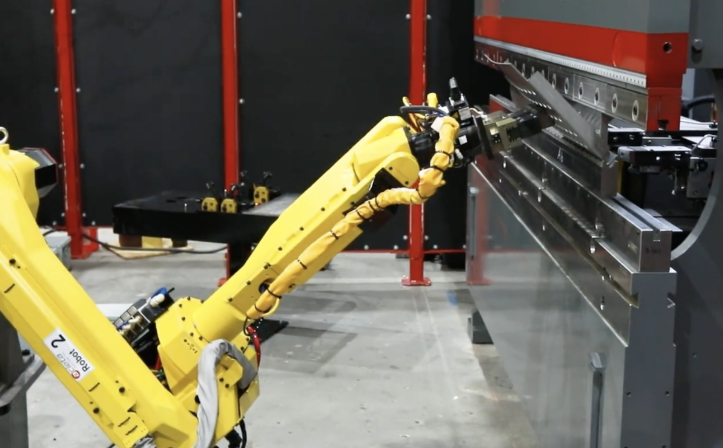
\includegraphics[width=0.85\textwidth]{figures/press_brake_system.png}
\caption{Robotic press brake bending system with integrated robot handling source -\cite{acieta_press_brake}}
\label{fig:press_brake_system}
\end{figure}

In automated bending systems, industrial robots are used to perform tasks such as picking the sheet, positioning it within the press brake, reorienting it for subsequent bending operations, and unloading the final part. Robotic integration enables improved repeatability and reduces operator dependency in high-volume production environments \cite{Aomura2002RoboticBending}.

\subsection{ Process Characteristics and Challenges}
A key characteristic of sheet metal bending is that the geometry of the workpiece changes after each bending operation. Unlike rigid object manipulation, the robot must continuously adapt to a dynamically evolving part shape. This directly affects, Grasp feasibility, Collision avoidance, Reachability constraints, Orientation planning.
Studies have shown that the feasibility of bending operations strongly depends on geometric constraints and tool accessibility, requiring careful coordination between robot motion and bending sequences\cite{Gupta1998SheetMetalBending}.
 
Another critical challenge is collision avoidance within constrained environments. The robot must operate in close proximity to the press brake tooling, which limits available workspace and increases the risk of collisions. Path planning methods must therefore consider both robot kinematics and environmental constraints\cite{Biagiotti2008Trajectory}.
Subsection{ Regripping and Workpiece Reorientation }
One of the most complex aspects of robotic sheet metal bending is the requirement for regripping operations. During multi-stage bending, the workpiece often needs to be repositioned to enable subsequent bends. This is typically achieved by placing the sheet at an intermediate location (e.g., orientation table) and re-grasping it in a new configuration.
Regrasp planning has been extensively studied in robotics and is typically formulated as a search problem over feasible grasp configurations and transitions between them \cite{wan2017regrasp}. However, in industrial bending applications, regripping is often implemented using predefined strategies, limiting flexibility when handling varying geometries \cite{Gupta1998SheetMetalBending}. 
In industrial bending applications, however, regripping is often implemented using predefined strategies due to process constraints. This limits flexibility and increases engineering effort when handling new geometries. As a result, regripping remains a major bottleneck in achieving fully automated bending systems \cite{Aomura2002RoboticBending}, \cite{Gupta1998SheetMetalBending}.
\subsection{ Grasping and Vacuum-Based Handling}
In many sheet metal applications, vacuum grippers are used due to their ability to handle flat surfaces efficiently. However, grasp stability becomes critical, especially when handling large or flexible sheets.
Research on vacuum-based gripping systems highlights the importance of modeling suction forces and ensuring sufficient contact area for stable manipulation\cite{VacuumGripperModeling}. Additionally, data-driven approaches to grasp synthesis have been proposed to improve robustness in uncertain environments \cite{Bogue2018}.
In bending processes, grasp selection must also consider future operations, ensuring that the chosen grasp does not interfere with subsequent bends or tool access. This introduces a coupling between grasp planning and process planning.
\subsection{ Trajectory Planning in Bending Environments }
Trajectory planning for robotic bending is significantly more complex than standard pick-and-place tasks due to workspace constraints and dynamic geometry changes. The robot must generate collision-free paths while maintaining feasible kinematic configurations.
 
Early research on robot-assisted bending highlighted the importance of path planning methods that account for both robot motion and process constraints\cite{Bogue2018}. These methods must ensure that the robot can safely move between intermediate positions, especially during reorientation and regripping operations.
Classical trajectory generation methods provide a foundation for generating smooth and feasible robot motion \cite{Biagiotti2008Trajectory}. However, these approaches often assume static environments and do not fully address the challenges introduced by changing workpiece geometry and constrained bending setups.

\subsection{ Limitations of Existing Industrial Systems }
Despite significant progress, existing robotic bending systems exhibit several limitations such as , Heavy reliance on predefined handling strategies,Limited adaptability to varying geometries,High engineering effort for process setup,Lack of integration between grasp planning, regrip planning, and trajectory generation
Many industrial systems use conservative motion planning to ensure safety, which reduces efficiency when handling complex parts. Additionally, most approaches treat grasping, planning, and execution as separate stages, leading to suboptimal performance.
\subsection{ Relevance to This Thesis }
The challenges identified in robotic sheet metal bending,particularly dynamic geometry handling, regripping, and constrained trajectory planning,directly motivate the approach developed in this thesis.
Unlike traditional systems, the proposed implementation integrates, Automated trajectory generation, Constraint-aware motion planning, Structured execution pipelines
This enables more flexible and scalable automation of bending operations, addressing key limitations identified in the state of the art.


\section{Manual and Teach Pendant Programming}
Manual robot programming using teach pendants represents one of the earliest and most widely adopted approaches in industrial robotics. In this method, robot motions are explicitly defined by an operator through direct interaction with the robot controller. The operator either guides the robot to desired positions or manually inputs Cartesian or joint coordinates, which are stored as waypoints and executed sequentially by the control system.
Figure~\ref{fig:teach_pendant} illustrates a typical teach pendant interface used for manual robot programming.
\begin{figure}[htbp]
\centering
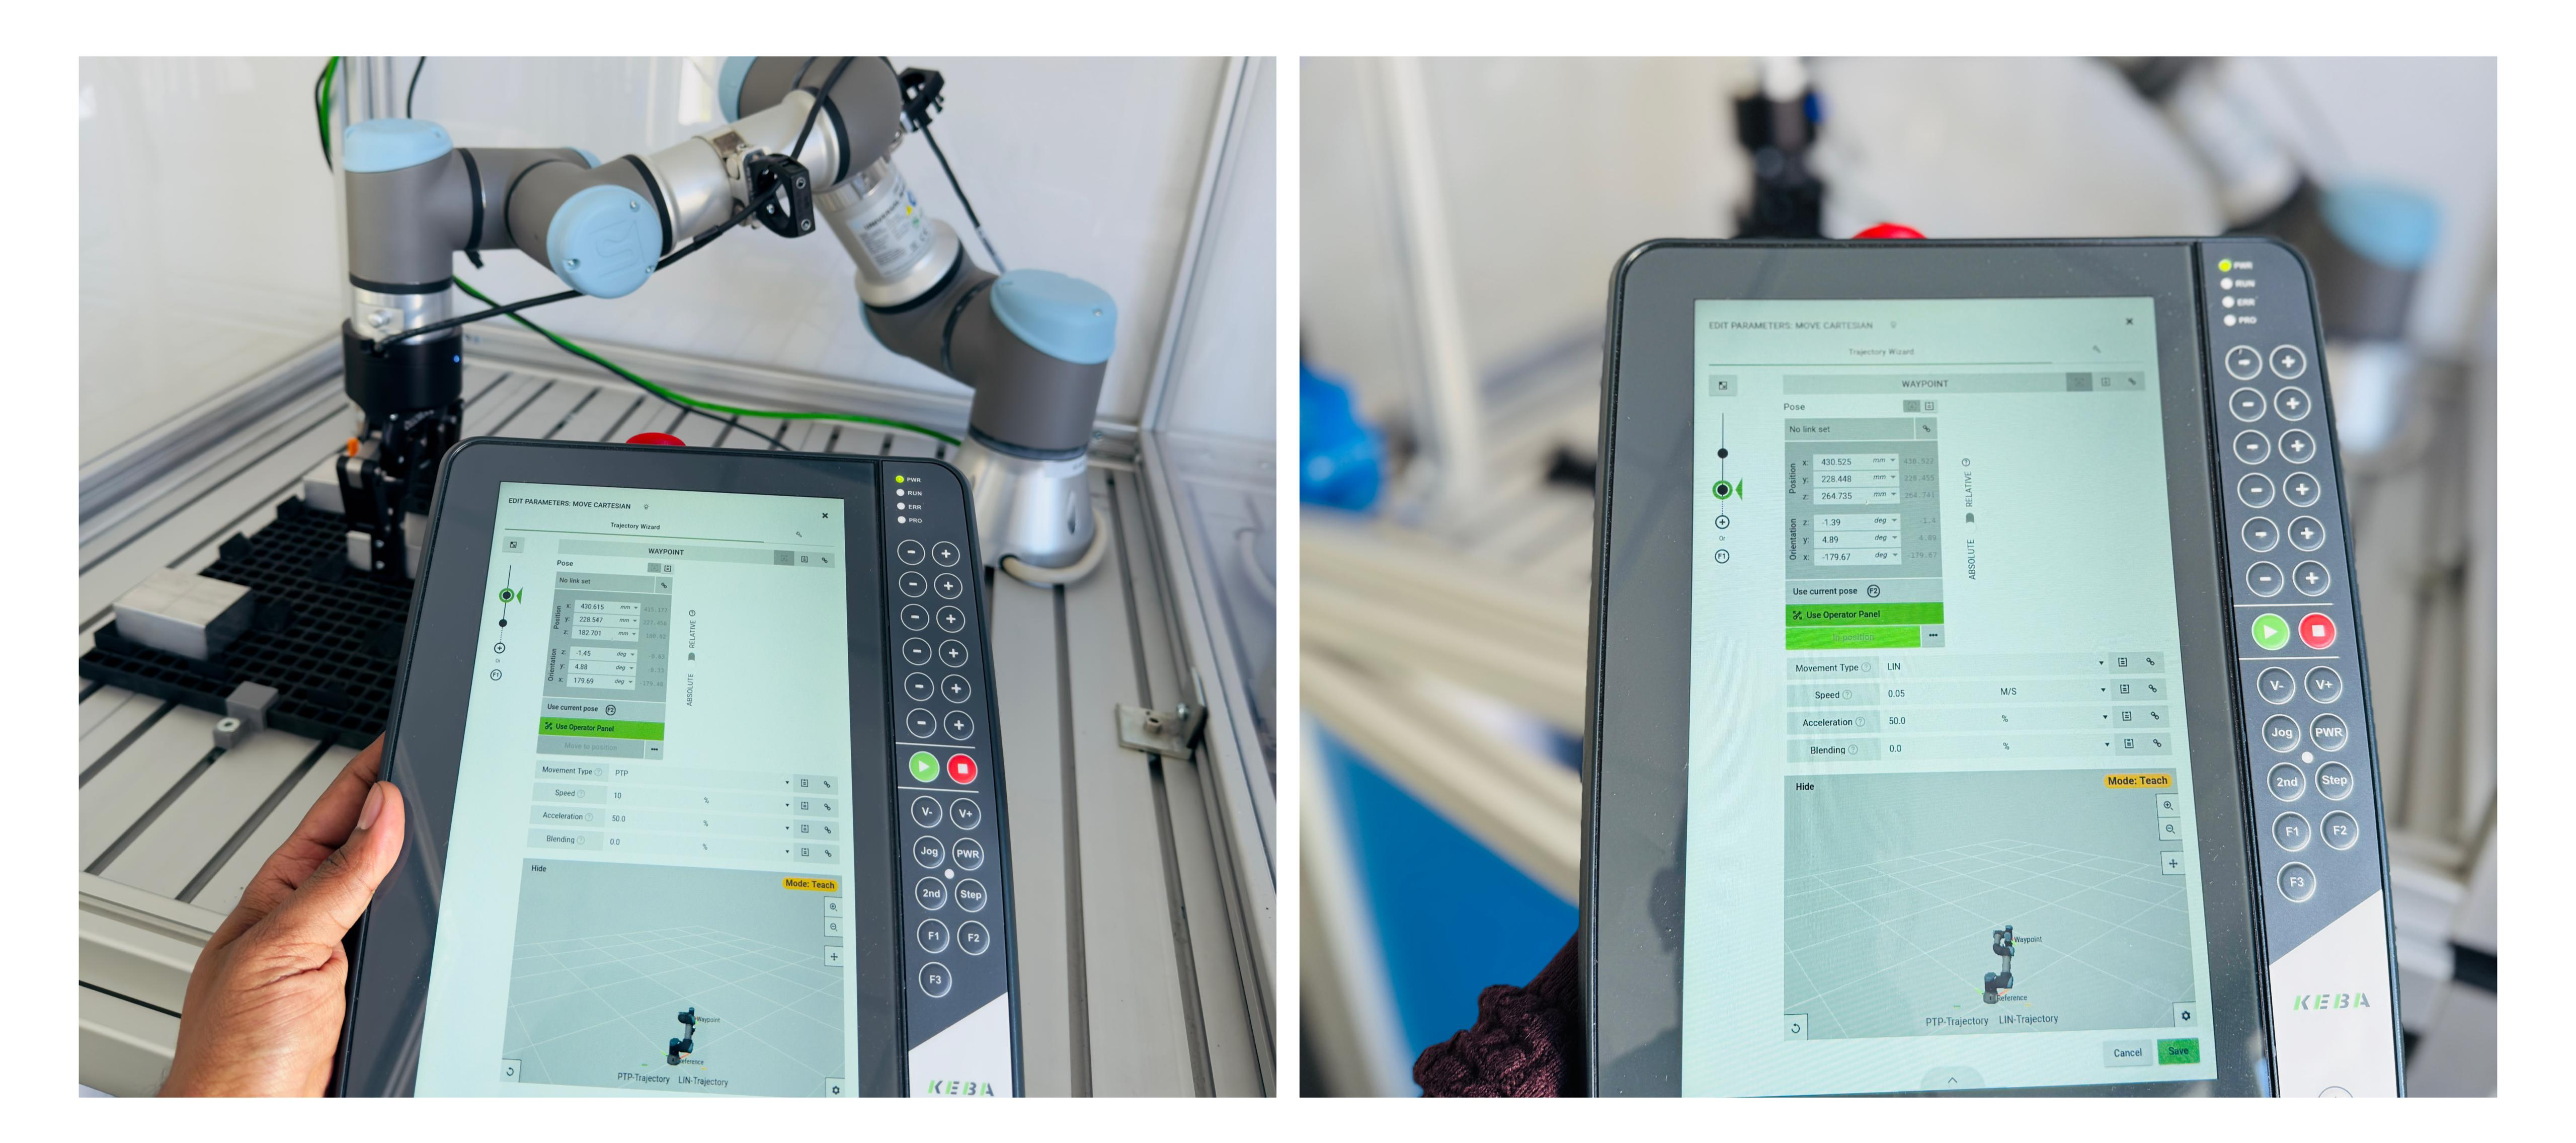
\includegraphics[width=0.75\textwidth]{figures/teach_pendant.png}
\caption{Teach pendant interface for manual robot programming (Source: Own work9)} 
\label{fig:teach_pendant}
\end{figure}
This programming approach provides a high level of control and is particularly suitable for structured and repetitive tasks. It allows operators to directly verify robot motions during programming, reducing the risk of unexpected behavior during execution. As a result, manual programming remains widely used in industrial environments where tasks are stable and do not require frequent modification \cite{Siciliano2016Robotics}.
\subsection{Limitations of Manual Programming}
Despite its advantages, manual programming exhibits several limitations, particularly in flexible manufacturing scenarios. One major drawback is the high dependency on operator expertise, as programming requires knowledge of robot kinematics, coordinate systems, and process constraints. This increases setup time and introduces variability depending on the skill level of the operator.
Another limitation is the lack of scalability. When product geometry changes, the entire sequence of waypoints must often be redefined manually. This makes manual programming inefficient for applications involving high product variability or frequent reconfiguration \cite{Bogue2018}.
Furthermore, manual programming does not inherently account for process constraints such as collision avoidance, reachability, or optimal path planning. These factors must be considered explicitly by the operator, increasing the complexity of programming and the likelihood of errors
\subsection{Challenges in Complex Manipulation Tasks}
In applications such as robotic sheet metal bending, manual programming becomes particularly challenging due to the need for multi-stage manipulation and reorientation. The operator must anticipate changes in workpiece geometry and define intermediate waypoints accordingly.
Additionally, regripping operations require careful coordination of placement and grasping actions, which are difficult to define manually in a consistent and scalable manner. As task complexity increases, the number of required waypoints grows significantly, leading to longer programming times and reduced efficiency.
These limitations highlight the inadequacy of manual programming for complex and dynamic industrial processes, where automation and adaptability are required.
\subsection{Transition Towards Automated Programming}
The limitations of manual programming have motivated the development of higher-level programming approaches, including offline programming and automatic program generation. These approaches aim to reduce reliance on operator intervention by generating robot motions based on process requirements and system constraints.
In modern industrial practice, there is a clear shift from manual programming towards automated and rule-based approaches, particularly in applications involving variable geometries and multi-stage processes. This transition forms the basis for the approaches discussed in the subsequent sections.
 
\section{Offline Programming Approaches for Industrial Robots}
Offline programming (OLP) is an established approach in industrial robotics that enables the development and validation of robot programs within a virtual environment prior to execution on physical systems. In contrast to manual programming, OLP decouples programming from production, allowing robot trajectories and task sequences to be generated without interrupting ongoing operations.
 
Figure~\ref{fig:olp_environment} illustrates a typical offline programming environment, where a virtual model of the robot, tooling, and workcell is used to simulate and validate motion trajectories.
 
\begin{figure}[htbp]
\centering
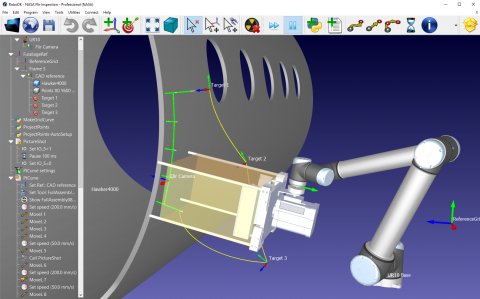
\includegraphics[width=0.85\textwidth]{figures/olp_environment.png}
\caption{Offline robot programming environment with CAD-based simulation (Source: \cite{RoboDK2024})}
\label{fig:olp_environment}
\end{figure}
Offline programming systems typically rely on CAD models and geometric representations of the robot and its environment. These models are used to simulate robot motion, evaluate reachability, and detect potential collisions before execution. This approach significantly reduces downtime and improves safety by allowing errors to be identified during the planning phase \cite{Chryssolouris2013}.
\subsection{Digital Twin and Simulation-Based Programming}
A key development in offline programming is the use of digital twins, which represent a virtual replica of the physical robotic system. Digital twin models enable real-time synchronization between the simulated environment and the physical system, allowing more accurate validation of robot programs.
Digital twin-driven manufacturing approaches have been widely studied, demonstrating their effectiveness in improving system reliability and reducing commissioning time \cite{Tao2019}. By incorporating sensor data and system feedback, digital twins can enhance the accuracy of simulation-based planning.
In industrial practice, simulation platforms such as Drag and bot  RoboDK, ABB RobotStudio, and KUKA.Sim provide comprehensive environments for offline programming, including path planning, collision detection, and code generation.
Advantages of Offline Programming compared to manual programming, which Reduced production downtime, as programming is performed outside the physical system, Improved safety due to collision detection and validation in simulation, Enhanced visualization, enabling operators to analyse robot motion before execution, Support for complex environments, where direct manual programming is difficult. These advantages make OLP a widely adopted solution in industrial automation, particularly for applications requiring precise and repeatable motion.
\subsection{ Limitations of Offline Programming}
Despite its benefits, offline programming has several limitations. One major challenge is the dependency on model accuracy. Any mismatch between the virtual model and the real environment can result in deviations during execution, requiring manual correction.
Furthermore, offline programming still relies heavily on manual input for defining trajectories and task sequences. Although simulation tools assist in validation, they do not inherently generate robot programs automatically. As a result, significant engineering effort is still required to adapt programs to new workpiece geometries or process changes \cite{Bogue2018}.
Another limitation is the lack of integration with higher-level task planning. In many systems, offline programming is used primarily for trajectory validation rather than for fully automated task generation. This limits its ability to handle dynamic and complex industrial  processes such as robotic sheet metal bending.
 While offline programming improves efficiency compared to manual programming, it does not eliminate the need for human intervention in defining robot motions. In applications involving dynamic geometry changes and multi-stage manipulation, such as sheet metal bending, these limitations become significant.
The approach developed in this thesis builds upon the advantages of simulation-based environments while addressing their limitations by introducing automated trajectory generation and constraint-aware motion planning. Unlike traditional offline programming, the proposed system generates robot trajectories programmatically and executes them through a structured pipeline, reducing reliance on manual programming.


\section{Automatic and Rule-Based Robot Program Generation}
Automatic robot programming aims to reduce or eliminate manual intervention by generating robot programs directly from high-level task descriptions, process parameters, or environmental inputs. Unlike manual and offline programming approaches, which require explicit definition of trajectories, automatic programming systems compute robot motions programmatically based on predefined rules, constraints, or models.
 
\subsection{Task-Level Programming and Abstraction}
A fundamental concept in automatic robot programming is task-level programming, where users specify what the robot should achieve rather than how it should move. The system then decomposes high-level tasks into sequences of executable actions.
Early work on robot programming introduced the concept of abstraction layers, enabling robot programs to be generated from symbolic descriptions of tasks \cite{LozanoPerez1983}. This approach reduces the need for detailed motion specification and allows systems to operate at a higher level of reasoning.
More recent research has focused on skill-based programming, where tasks are represented as reusable motion primitives or skills. These skills encapsulate common operations such as grasping, placing, or approaching, and can be combined to form complex task sequences \cite{Kruger2019}. This modular approach improves scalability and reusability in industrial applications.

\subsection{Rule-Based and Constraint-Based Planning}
 
In structured industrial environments, automatic programming is often implemented using rule-based systems, where robot behaviour is defined through a set of logical rules and constraints. These rules govern decisions such as grasp selection, motion sequencing, and collision avoidance.
Constraint-based approaches extend this concept by incorporating geometric, kinematic, and process constraints into the planning process. The system evaluates feasible solutions based on these constraints and generates valid robot trajectories accordingly.
Such approaches are particularly effective in applications where process conditions are well-defined, enabling deterministic and reliable program generation. However, the complexity of rule sets increases significantly with task variability, making system design and maintenance more challenging \cite{Villani2018}.
 
A key challenge in automatic robot programming is the integration of multiple planning components, including Grasp planning, Regrip planning, Trajectory generation, Collision avoidance.
In many existing systems, these components are developed independently, resulting in fragmented workflows and limited adaptability. For example, grasp planning methods may not consider future trajectory constraints, leading to infeasible execution scenarios.
Research in robotic manipulation highlights the importance of integrating these components into a unified framework to achieve robust and efficient task execution \cite{bohg2014data}. However, achieving such integration in industrial environments remains an open challenge due to the complexity of real-world constraints.
Despite significant advancements, current automatic programming approaches exhibit several limitations: such as, Limited integration between planning modules, grip position finding for changing workpiece geometry, collsion avoidance, Scalability issues in rule-based systems, Dependency on structured environments, Insufficient adaptability to dynamic geometry changes.
These limitations are particularly evident in applications such as robotic sheet metal bending, where the workpiece geometry evolves during the process and requires continuous adaptation of robot actions. 
The limitations identified in automatic robot programming directly motivate the approach developed in this thesis. While existing methods provide partial automation, they do not fully integrate all required planning components into a unified pipeline.
The proposed system addresses this gap by, combining trajectory generation, constraint handling, and execution into a structured workflow, generating robot motions automatically from validated target poses, Reducing reliance on manual programming and predefined rules
This integrated approach enables more flexible and scalable automation, particularly in complex applications such as robotic sheet metal bending.
 



